\subsection{Feldorientierte Regelung (FOC)}\label{Feldorientierte Regelung}
	Mithilfe der feldorientiereten Regelung ist es m�glich das Feld des Stators so anzupassen, dass es dem Feld des Rotors genau so vorl�uft, dass Drehmoment und Effizienz maximiert werden. Im Gegensatz zur BLDC-Regelung kann das Statorfeld nicht nur 6 Positionen annehmen, sondern unbegrenzt viele. Man kann mit dieser Methode auch eine etwas h�here Drehzahl erreichen. Um diese 90� Verschiebung des Statorfelds zu erreichen, wird der Feldvektor zun�chst in seine zwei Komponenten Id und Iq aufgeteilt:
	
	\begin{figure}[H]
			\centering
			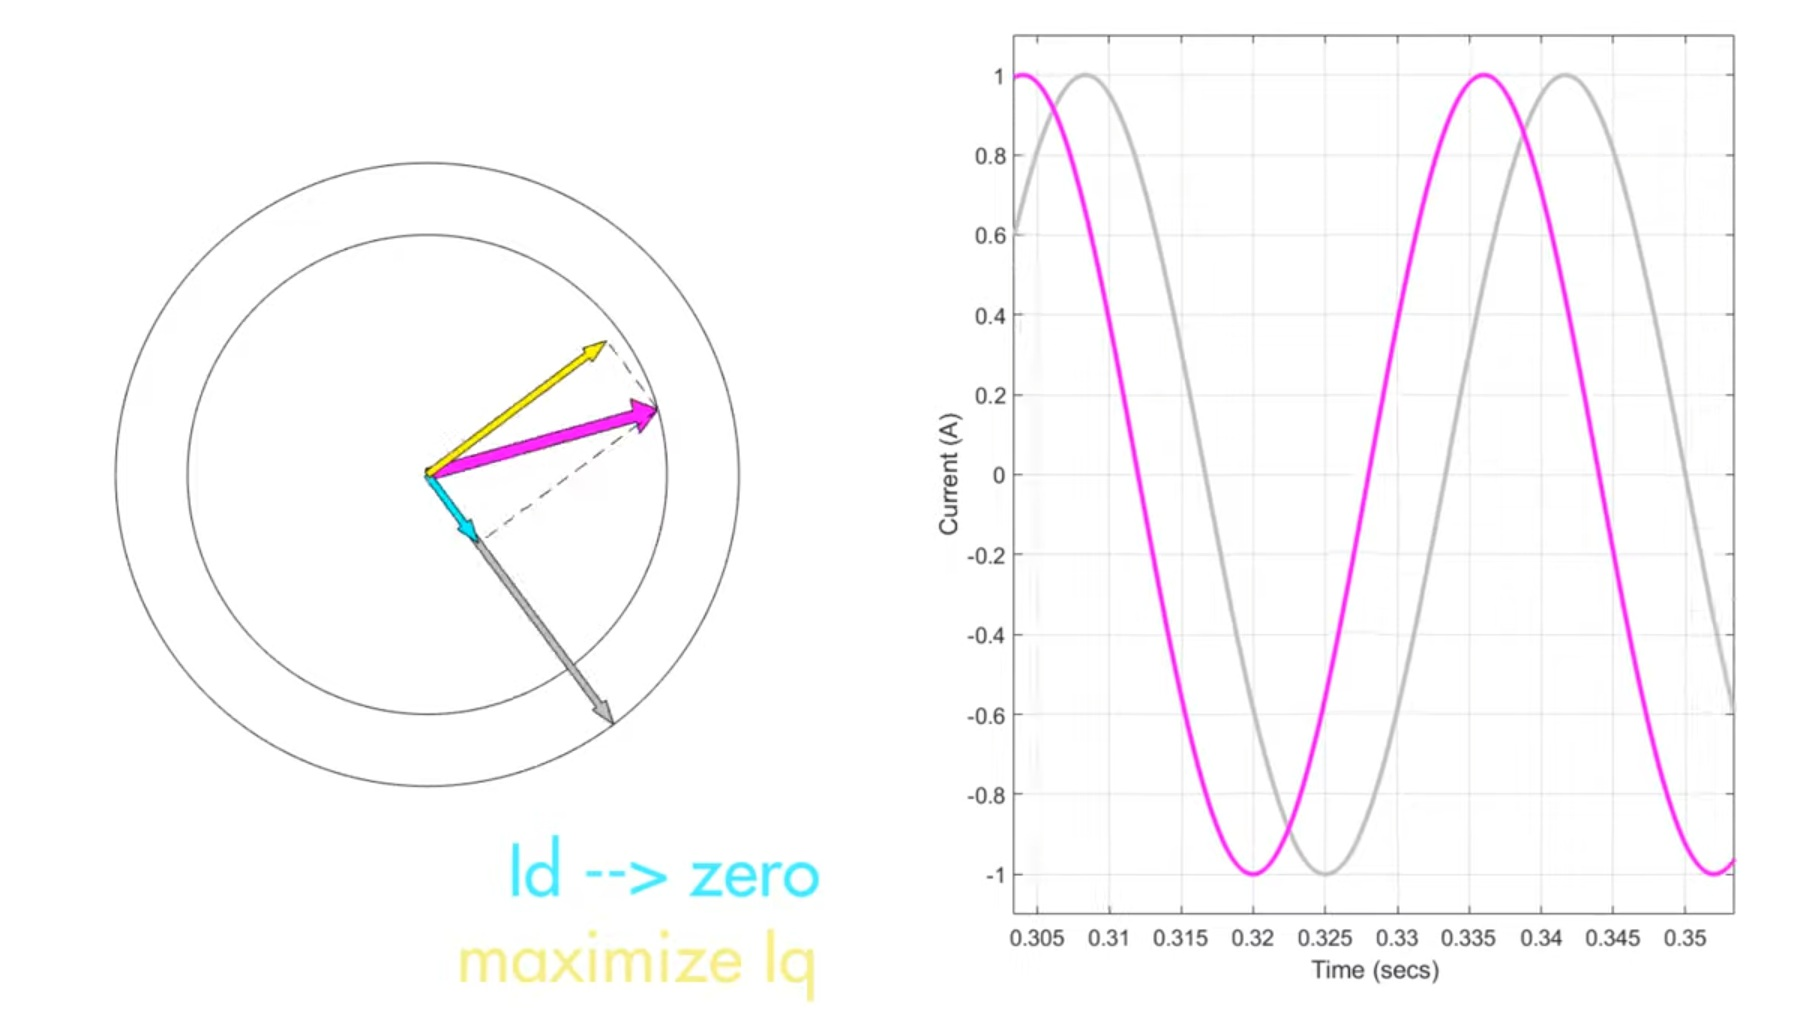
\includegraphics[scale=0.3]{./3_Stand_der_Technik/Abbildungen/FOC_Control_1}
			\caption{Komponenten des Statormagnetfelds\cite{MATLAB2020}}
	\end{figure}
	
	Das Ziel des Reglers ist demnach Id gegen 0 zu regeln und Iq entsprechend dem gew�nschten Drehmoment so hoch wie m�glich zu regeln.
	
	Der Aufbau eines FOC-Algorhitmus ist in der Regel wiefolgt:
	
	\begin{figure}[H]
			\centering
			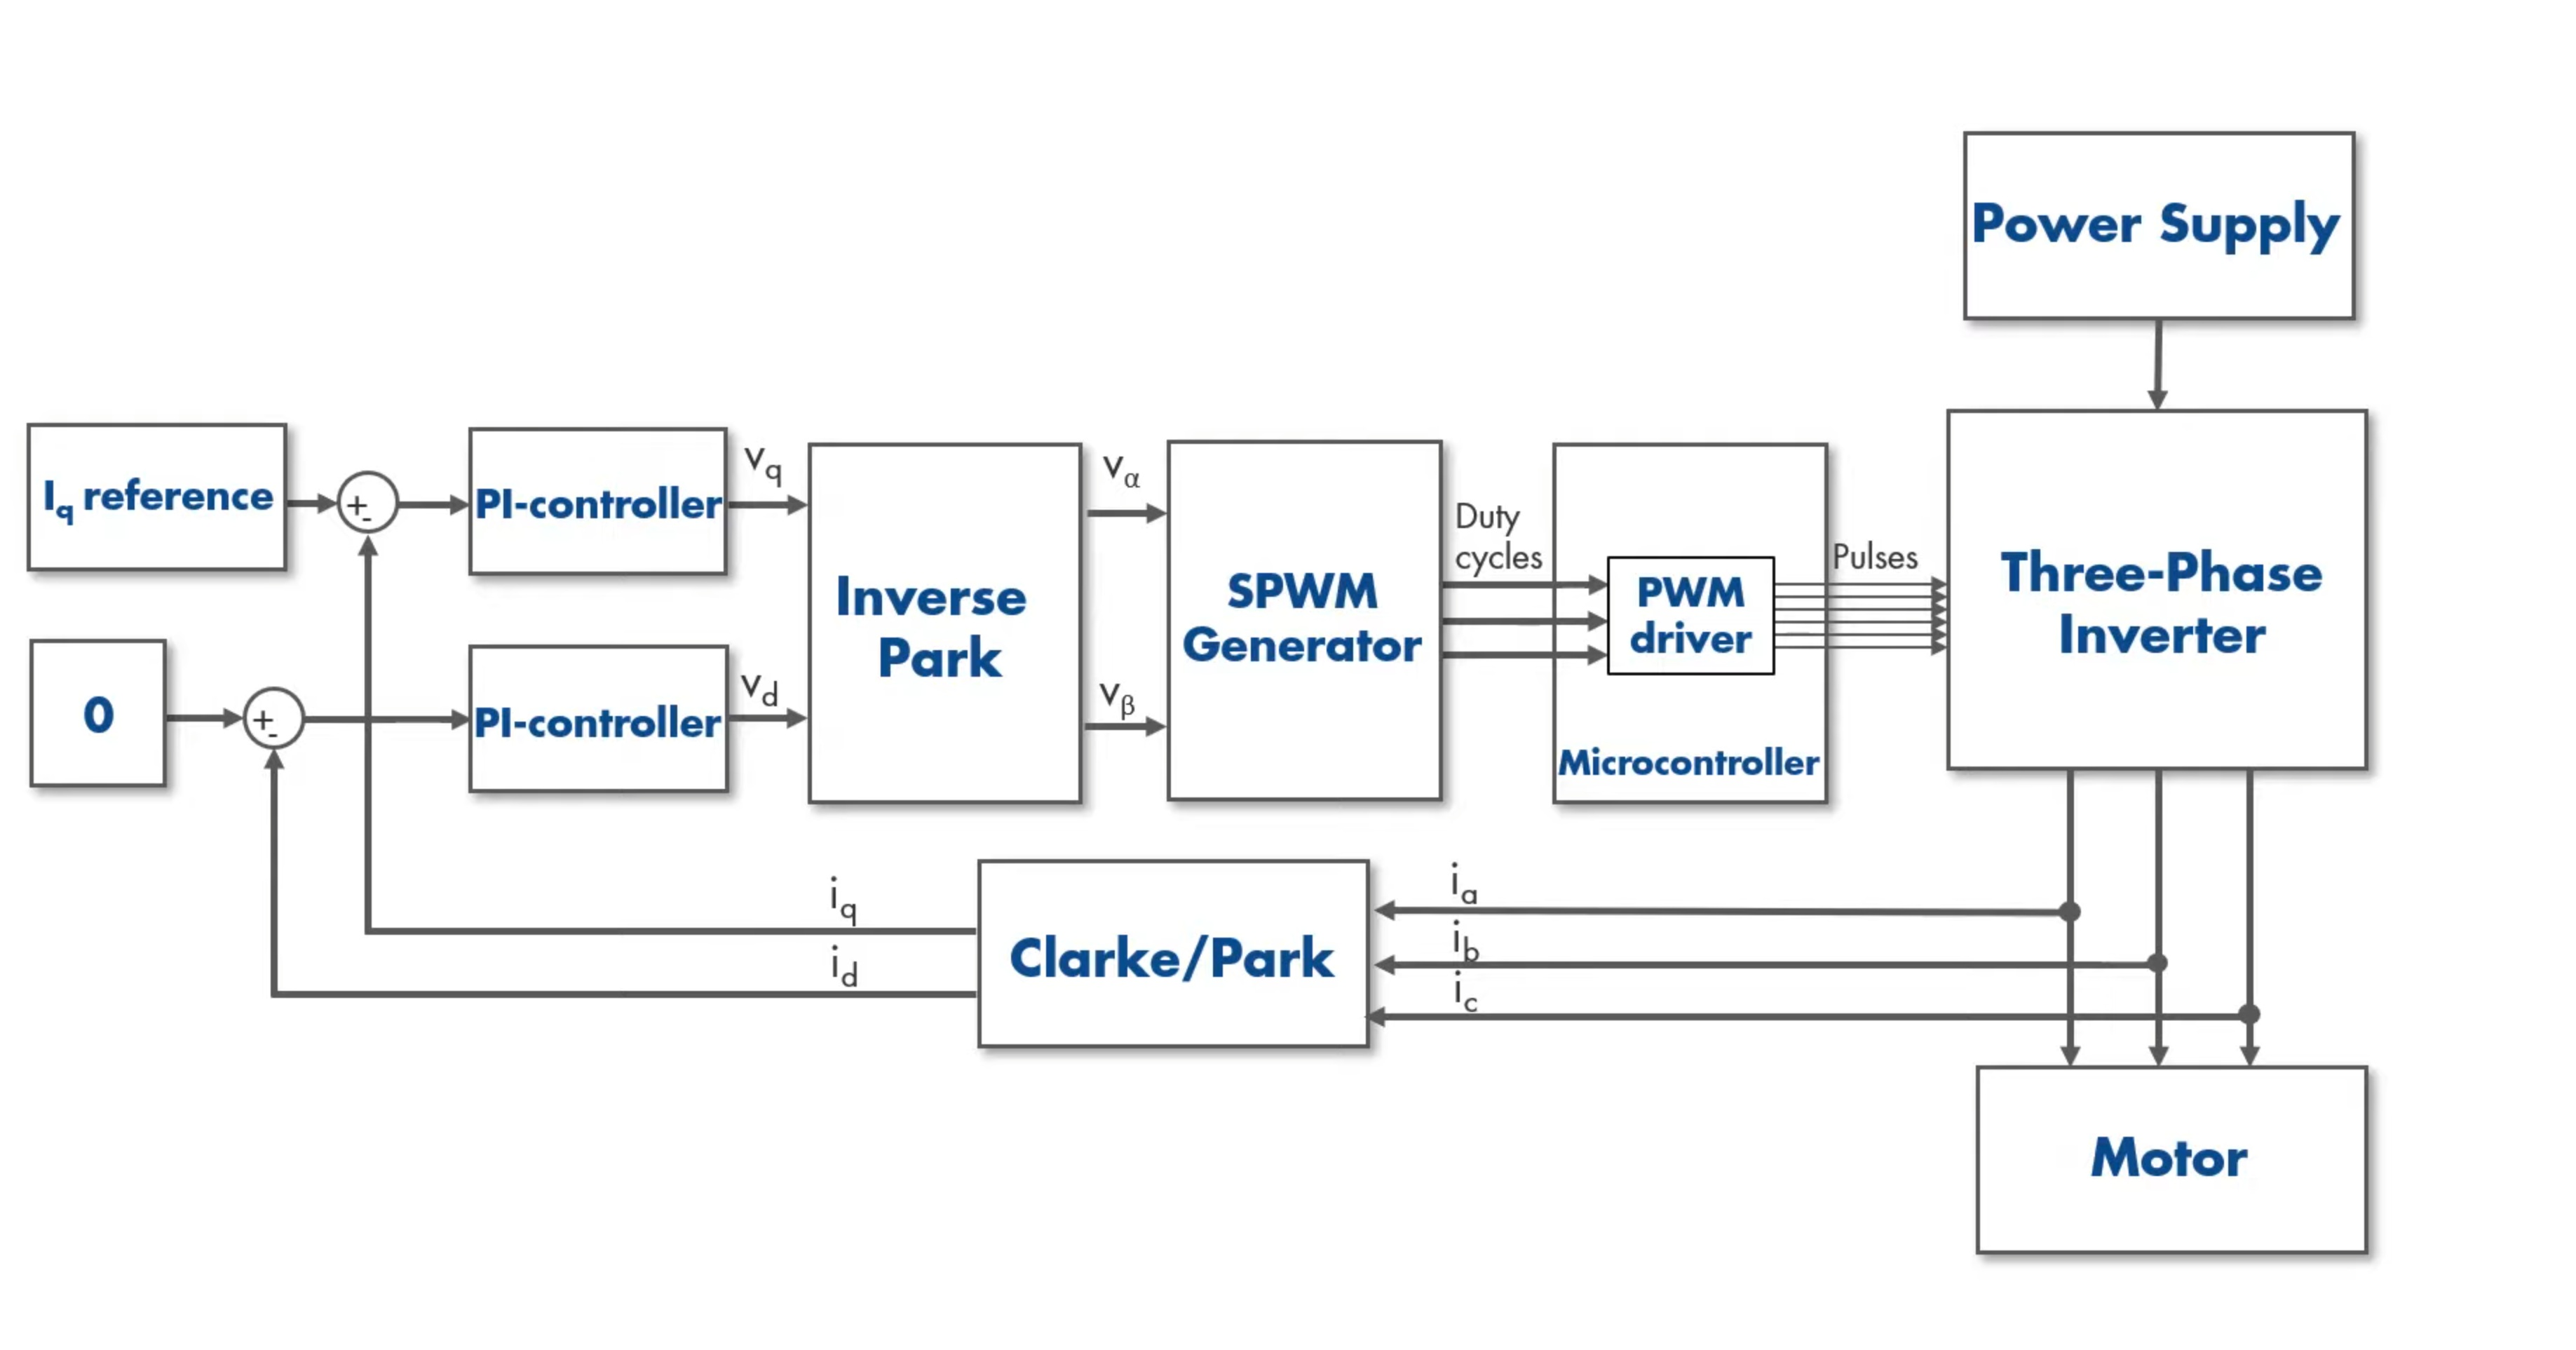
\includegraphics[scale=0.3]{./3_Stand_der_Technik/Abbildungen/FOC_Control_2}
			\caption{Aufbau eines FOC-Algorhitmus\cite{MATLAB2021}}
	\end{figure}
	
	Mithilfe von Shunts wird der derzeitige Strom zum Motor gemessen. Diese Werte werden mithilfe von mathematischen Transformationen (Clark- und Park Transformation) in die zwei Anteile Id und Iq aufgeteilt. Auch wird mithilfe eines Positionssensors die Position des Rotors gemessen.
	Zwei PI-Regler regeln nun Id auf 0 und Iq auf den gew�nschten Strom. Anschlie�end werden die Werte mithilfe von mathematischen Transformationen(inverse Clark Transformation) in die gew�nschten Spannungswerte Vd und Vq umgerechnet. 